% Updated versions of all figures and tables of poverty.tex and SM.tex with the September 2026 PIP data (2021 PPP).
% Figures and tables are generated by code_poverty/paper_update.R (after code_poverty/update.R).
\documentclass[12pt,english]{article}
\usepackage[utf8]{inputenc}
\usepackage{tgpagella}
\usepackage{mathpazo}
\usepackage[left=1in,right=1in,top=1in,bottom=1in]{geometry}
\usepackage[natbibapa]{apacite}
\bibliographystyle{apacite}
\usepackage{url}
\usepackage{xcolor}
\usepackage{hyperref}
\hypersetup{colorlinks=true, urlcolor=purple, linkcolor=blue, citecolor=violet}
\usepackage{babel}
\usepackage{booktabs}
\usepackage{makecell}
\usepackage{caption}
\usepackage{subcaption}
\usepackage{float}
\usepackage{graphicx}
\usepackage{amssymb}
\usepackage{placeins}
\setcitestyle{aysep={}}

% Generated by code_poverty/update.R on 2026-10-20
\newcommand{\upRatePovNow}{10.0}
\newcommand{\upRatePovThree}{7.1}
\newcommand{\upRatePovTrend}{8.5}
\newcommand{\upRatePovSeven}{3.8}
\newcommand{\upRatePovSDG}{1.6}
\newcommand{\upRatePovRealized}{7.6}
\newcommand{\upGapNow}{0.49}
\newcommand{\upGapThree}{0.28}
\newcommand{\upGapRealized}{0.31}
\newcommand{\upShareSurveyRecent}{63}
\newcommand{\upNbCountries}{171}
\newcommand{\upNbCapEight}{8}
\newcommand{\upCountriesCapEight}{Burundi, Central African Republic, D.R. Congo, Madagascar, Malawi, Mozambique, South Sudan and Zambia}
\newcommand{\upNbCapEightRealized}{11}
\newcommand{\upNbCapEightLIC}{8}
\newcommand{\upTaxEightSSA}{85}
\newcommand{\upTaxEightLIC}{129}
\newcommand{\upTaxEightNGA}{38}
\newcommand{\upCapSevenCOD}{5.8}
\newcommand{\upCapSevenBDI}{10.0}
\newcommand{\upMeanThreeMDG}{3.7}
\newcommand{\upNbMeanBelowThree}{1}
\newcommand{\upCountriesMeanBelowThree}{D.R. Congo}
\newcommand{\upTaxEighteenSevenIND}{0}
\newcommand{\upTaxEighteenTrendIND}{0}
\newcommand{\upTaxEighteenThreeIND}{2.3}
\newcommand{\upTaxEighteenRealizedIND}{0.12}
\newcommand{\upRateThreeIND}{1.0}
\newcommand{\upTrendIND}{5.5}
\newcommand{\upNbFloor}{31}
\newcommand{\upNbFloorLIC}{19}
\newcommand{\upNbFloorSeven}{13}
\newcommand{\upNbFloorSevenHFCE}{10}
\newcommand{\upNbFloorSDG}{5}
\newcommand{\upCountriesFloorSDG}{Central African Republic, D.R. Congo, Mozambique, South Sudan and Zambia}
\newcommand{\upNbFloorRealized}{30}
\newcommand{\upFloorETH}{2.4}
\newcommand{\upFloorNGA}{2.1}
\newcommand{\upGlobalFloor}{9.4}
\newcommand{\upGiniThree}{0.61}
\newcommand{\upGiniThreeGlobalTax}{0.50}
\newcommand{\upRateHundred}{2.2}
\newcommand{\upRateHundredHFCE}{0.51}
\newcommand{\upShareBelowHundred}{95}
\newcommand{\upEqLine}{2.5}
\newcommand{\upEqThreshold}{7.8}
\newcommand{\upRatePovNowEq}{6.8}
\newcommand{\upRatePovThreeEq}{4.8}
\newcommand{\upRatePovSevenEq}{2.6}
\newcommand{\upRatePovSDGEq}{1.0}
\newcommand{\upRatePovRealizedEq}{5.2}
\newcommand{\upGapThreeEq}{0.15}
\newcommand{\upNbCapEq}{7}
\newcommand{\upCountriesCapEq}{Burundi, Central African Republic, D.R. Congo, Malawi, Mozambique, South Sudan and Zambia}
\newcommand{\upTaxEqSSA}{47}
\newcommand{\upTaxEqLIC}{72}
\newcommand{\upTaxEqNGA}{15.8}
\newcommand{\upTaxEighteenThreeINDEq}{0}
\newcommand{\upNbFloorEq}{19}
\newcommand{\upNbFloorSevenEq}{9}
\newcommand{\upNbFloorSDGEq}{2}
\newcommand{\upRateHundredEq}{1.2}
\newcommand{\upGlobalFloorEq}{9.5}
\newcommand{\upRatePovThreeTF}{5.7}
\newcommand{\upRatePovSevenTF}{2.1}
\newcommand{\upRatePovRealizedTF}{6.2}
\newcommand{\upGapThreeTF}{0.20}
\newcommand{\upNbCapTF}{7}
\newcommand{\upCountriesCapTF}{Burundi, Central African Republic, D.R. Congo, Malawi, Mozambique, South Sudan and Zambia}
\newcommand{\upTaxSSATF}{48}
\newcommand{\upNbFloorTF}{21}
\newcommand{\upNbFloorSevenTF}{7}
\newcommand{\upRatePovThreeTFEq}{3.8}
\newcommand{\upRatePovSevenTFEq}{1.4}
\newcommand{\upRatePovRealizedTFEq}{4.2}
\newcommand{\upGapThreeTFEq}{0.11}
\newcommand{\upNbCapTFEq}{1}
\newcommand{\upCountriesCapTFEq}{D.R. Congo}
\newcommand{\upTaxSSATFEq}{26}
\newcommand{\upNbFloorTFEq}{13}
\newcommand{\upNbFloorSevenTFEq}{3}
\newcommand{\upRateHundredTF}{1.2}

% Generated by code_poverty/paper_update.R on 2026-10-21
\newcommand{\appKenyaCap}{10.2}
\newcommand{\appKenyaTax}{74}
\newcommand{\appKenyaFloor}{2.5}


\title{Shortfall of Domestic Resources to Eradicate Extreme Poverty by 2030:\\ Updated Figures and Tables with the September 2026 PIP Data}
\author{Adrien Fabre\thanks{CNRS, CIRED. E-mail: adrien.fabre@cnrs.fr.}}
\date{\today}

\begin{document}
\maketitle

\noindent This document provides updated versions of all figures and tables of \cite{fabre_shortfall_2025} and of its Supplementary Material, using the September 2026 vintage of the World Bank's Poverty and Inequality Platform (2021 PPP). The method is described in the accompanying note (\texttt{update.pdf}). Lines and thresholds are converted as follows: \$2.15/day becomes \$3.00/day (extreme poverty), \$3.65 becomes \$4.20 (severe poverty), \$6.85 becomes \$8.30 (acute poverty), and \$18.15/day (the U.S. poverty line) is unchanged. In all scenarios, incomes grow at the observed rate up to 2025 (or the survey year if later), and then at the scenario's rate. The scenario of 7\% growth starting in 2016 is not updated, as it would contradict the use of observed growth. ``HFCE rescaling'' refers to the robustness check in which survey data are rescaled to household final consumption expenditure from national accounts. The original figures are numbered in parentheses.

\section{Main text}

\begin{table}[h]

\caption[Global poverty (rates and gaps) in 2030 under different growth scenarios (September 2026 PIP data).]{\label{tab:poverty_update}Global poverty rates and poverty gaps in 2030 under different growth scenarios, using the September 2026 PIP data. Growth scenarios apply from 2025 (or the survey year if later), after observed growth. Poverty rates are expressed in \% of world population and poverty gaps in \% of world GDP. Poverty lines are in 2021 PPP \$/day.}
\centering
\begin{tabular}[t]{lrrrrrrrr}
\toprule Growth scenario & \multicolumn{4}{c}{Poverty rate (\%)} & \multicolumn{4}{c}{Poverty gap (\% of GDP)} \\ 
 (Poverty line in \$/day)  & 3.00 & 4.20 & 8.30 & 18.15 & 3.00 & 4.20 & 8.30 & 18.15\\
\midrule
2022 estimate & 10.0 & 19.0 & 47.9 & 71.6 & 0.49 & 1.32 & 8.36 & 38.30\\
2025 estimate & 9.2 & 16.2 & 43.8 & 69.5 & 0.44 & 1.13 & 6.91 & 33.83\\
Trend (2015--2025) & 8.9 & 14.4 & 37.5 & 66.1 & 0.41 & 0.99 & 5.35 & 27.79\\
Max(Trend, 0) & 8.5 & 14.1 & 37.3 & 66.0 & 0.38 & 0.94 & 5.25 & 27.62\\
Autoregressive projection & 8.5 & 14.4 & 39.8 & 67.3 & 0.37 & 0.96 & 5.70 & 29.47\\
3\% growth & 7.6 & 13.3 & 38.5 & 66.6 & 0.31 & 0.81 & 5.08 & 27.21\\
3\% unbalanced growth & 7.2 & 12.5 & 35.5 & 65.7 & 0.31 & 0.79 & 4.71 & 26.19\\
7\% growth & 5.2 & 9.5 & 29.5 & 61.0 & 0.17 & 0.47 & 3.04 & 18.87\\
\bottomrule
\end{tabular}
\end{table}

\begin{figure}[H]
  \caption[Idealized redistributive policies]{(Figure 1) Example of idealized redistributive policies: Kenya in 2030 after observed growth to 2025, then 3\% growth.}\label{fig:kenya_update}
  \begin{subfigure}{.5\textwidth}
    \caption[]{Consumption before/after idealized policies.}
    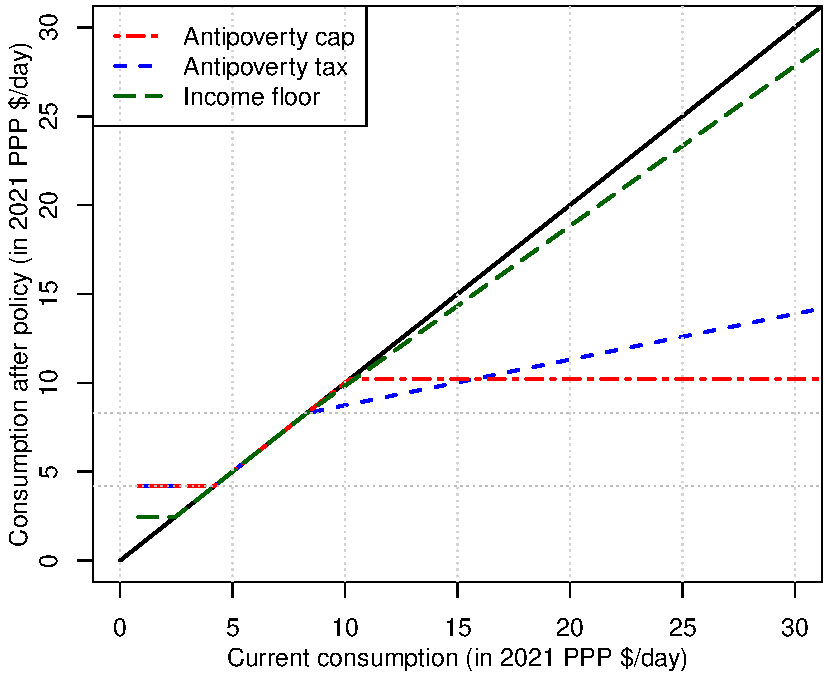
\includegraphics[width=\textwidth]{../figures/update/Kenya_policies.pdf}
  \end{subfigure} \;
  \begin{subfigure}{.5\textwidth}
    \caption[]{Anti-\textit{\$4.20-poverty} cap: \$\appKenyaCap/day.}
    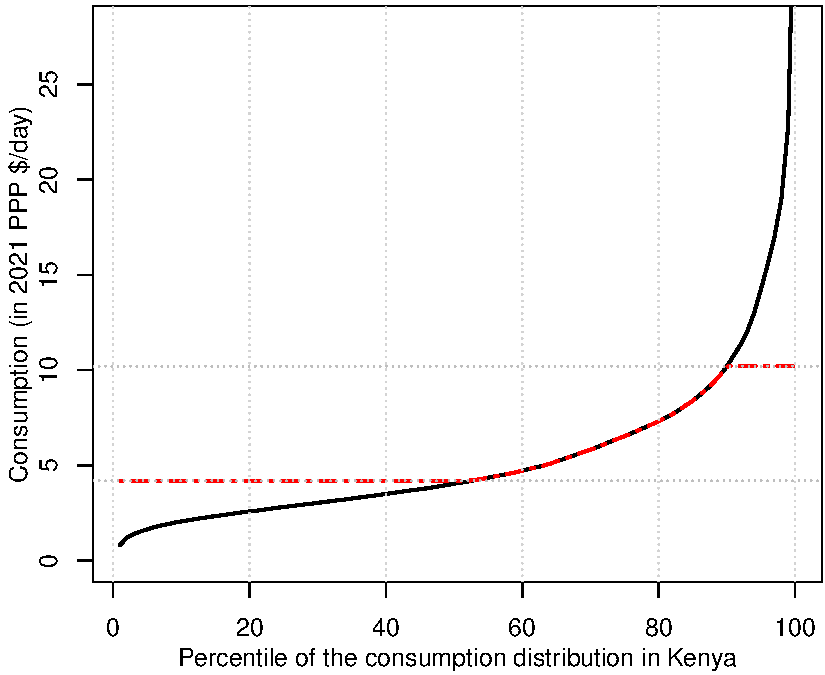
\includegraphics[width=\textwidth]{../figures/update/Kenya_cap.pdf}
  \end{subfigure}
  \\ \quad \\
  \begin{subfigure}{.5\textwidth}
    \caption[]{Anti-\textit{\$4.20-poverty} tax (above \$8.30/day): \appKenyaTax\%.}
    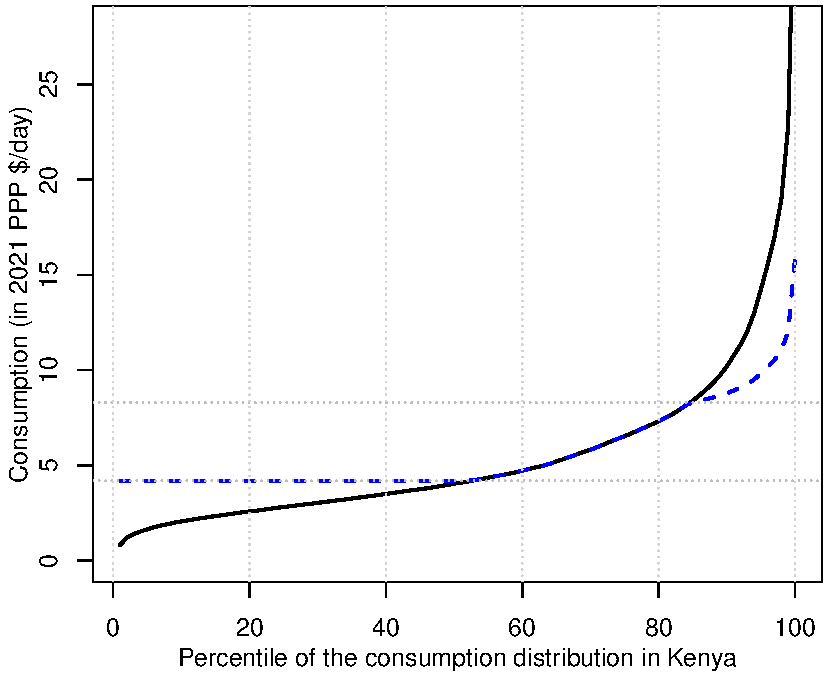
\includegraphics[width=\textwidth]{../figures/update/Kenya_tax.pdf}
  \end{subfigure} \;
  \begin{subfigure}{.5\textwidth}
    \caption[]{Income floor (funded by a 10\% tax above \$8.30/day): \$\appKenyaFloor/day.}
    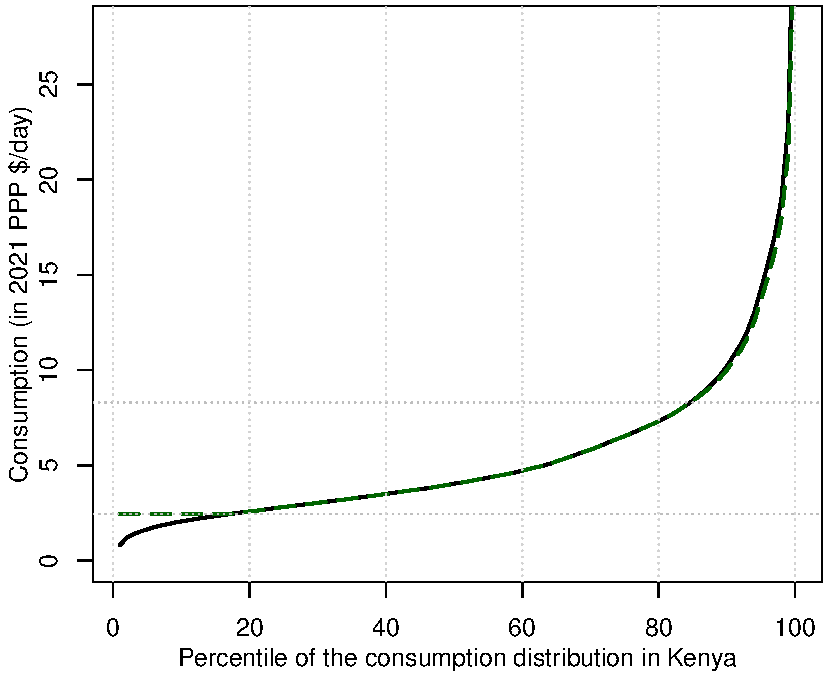
\includegraphics[width=\textwidth]{../figures/update/Kenya_floor.pdf}
  \end{subfigure}
\end{figure}

\newcommand{\mapfig}[3]{\begin{figure}[H]\caption{#2}\label{fig:#1_update}\makebox[\textwidth][c]{\includegraphics[width=1.1\textwidth]{../figures/update/#1.pdf}}#3\end{figure}}
\newcommand{\growththree}{after observed growth to 2025, then 3\% growth}
\newcommand{\growthseven}{after observed growth to 2025, then 7\% growth}

\mapfig{antipoverty_3_cap_average}{(Figure 2) Income cap eradicating extreme poverty (in 2021 PPP \$/day) in 2030, \growththree. All income above the cap is transferred to the extreme poor and lifts them to \$3.00/day.}{}
\mapfig{antipoverty_3_tax_8_average}{(Figure 3) Linear tax rate above \$8.30/day eradicating extreme poverty (in \%) in 2030, \growththree. All tax revenue is transferred to the extreme poor and lifts them to \$3.00/day.}{}
\mapfig{antipoverty_3_tax_18_very_optimistic}{(Figure 4) Linear tax rate above \$18.15/day eradicating extreme poverty (in \%) in 2030, \growthseven.}{}
\mapfig{floor_8__10}{(Figure 5) Income floor that can be funded with a 10\% marginal tax on income above \$8.30/day (in 2021 PPP \$/day) in 2030, \growththree.}{}

\FloatBarrier
\section{Supplementary Material: figures}

\mapfig{s_antipoverty_3_tax_8_average}{Linear tax rate above \$8.30/day eradicating extreme poverty (in \%), with HFCE rescaling, in 2030, \growththree.}{}
\mapfig{antipoverty_3_tax_8_reg}{Linear tax rate above \$8.30/day eradicating extreme poverty (in \%) in 2030, after observed growth to 2025, then growth predicted by the autoregressive projection.}{}
\mapfig{antipoverty_3_tax_18_average}{Linear tax rate above \$18.15/day eradicating extreme poverty (in \%) in 2030, \growththree.}{}
\mapfig{s_antipoverty_3_tax_18_very_optimistic}{Linear tax rate above \$18.15/day eradicating extreme poverty (in \%), with HFCE rescaling, in 2030, \growthseven.}{}
\mapfig{antipoverty_4_tax_18_average}{Linear tax rate above \$18.15/day eradicating severe poverty (at \$4.20/day, in \%) in 2030, \growththree.}{}
\mapfig{antipoverty_8_tax_18_average}{Linear tax rate above \$18.15/day eradicating acute poverty (at \$8.30/day, in \%) in 2030, \growththree.}{}
\mapfig{antipoverty_8_tax_8_average}{Linear tax rate above \$8.30/day eradicating acute poverty (at \$8.30/day, in \%) in 2030, \growththree. As the poverty line equals the taxation threshold, the rate exceeds 100\% wherever the poverty gap exceeds the taxable base.}{}
\mapfig{floor_8__10_very_optimistic}{Income floor that can be funded with a 10\% marginal tax on income above \$8.30/day (in 2021 PPP \$/day) in 2030, \growthseven.}{}
\mapfig{s_floor_8__10}{Income floor that can be funded with a 10\% marginal tax on income above \$8.30/day (in 2021 PPP \$/day), with HFCE rescaling, in 2030, \growththree.}{}

\FloatBarrier
\section{New figures}

\mapfig{antipoverty_3_cap_very_optimistic}{Income cap eradicating extreme poverty (in 2021 PPP \$/day) in 2030, \growthseven.}{}
\mapfig{mean_Y3}{Mean consumption (or income) per capita (in 2021 PPP \$/day) in 2030, \growththree.}{}
\mapfig{antipoverty_3_tax_8_average_2035}{Linear tax rate above \$8.30/day eradicating extreme poverty (in \%) in 2035, \growththree.}{}
\mapfig{antipoverty_3_tax_8_very_optimistic_2035}{Linear tax rate above \$8.30/day eradicating extreme poverty (in \%) in 2035, \growthseven.}{}
\mapfig{floor_8__10_2035}{Income floor that can be funded with a 10\% marginal tax on income above \$8.30/day (in 2021 PPP \$/day) in 2035, \growththree.}{}

\FloatBarrier
\section{Supplementary Material: tables}
Major lower-income countries are those with more than 10 million inhabitants and a mean consumption below \$8.40/day (the 2021-PPP counterpart of the original cut-off of \$6/day). Regional rows aggregate the distributions of all countries of the region.

\begin{table}[h]

\caption[Mean income in different scenarios, survey years and HFCE ratio (update).]{\label{tab:income_update}Mean income in major lower-income countries in various years and growth scenarios, survey years and ratio of HFCE (national accounts) to survey mean (September 2026 PIP data, 2021 PPP).}
\centering\footnotesize
\makebox[\textwidth][c]{
\begin{tabular}[t]{lrrrrrrrrr}
\toprule  & Year & \multicolumn{7}{c}{Mean consumption/income (in \$/day)} & HFCE to \\ 
 & of & year of & 2022 & 2025 & \multicolumn{4}{c}{2030 estimate} & survey \\ 
 & survey & survey & est. & est. & 3\% & 7\% & Projection & Trend & ratio \\ 
\midrule
World & 2022 & 20.0 & 19.8 & 21.3 & 24.7 & 30.1 & 23.4 & 24.0 & 1.46\\
Low-Income Countries & 2020 & 3.9 & 3.8 & 3.9 & 4.7 & 6.0 & 4.3 & 4.3 & 1.10\\
Sub-Saharan Africa & 2020 & 4.7 & 4.7 & 4.9 & 5.7 & 6.9 & 5.3 & 5.1 & 1.35\\
\midrule Angola & 2018 & 6.2 & 5.4 & 5.4 & 6.2 & 7.5 & 5.6 & 4.7 & 1.62\\
Bangladesh & 2022 & 7.5 & 7.5 & 8.3 & 9.6 & 11.6 & 9.4 & 10.5 & 1.90\\
Benin & 2021 & 5.3 & 5.5 & 6.3 & 7.3 & 8.8 & 6.8 & 7.4 & 1.21\\
Burkina Faso & 2021 & 4.5 & 4.4 & 4.7 & 5.5 & 6.6 & 5.1 & 5.3 & 0.96\\
Burundi & 2020 & 2.6 & 2.6 & 2.7 & 3.1 & 3.8 & 2.9 & 2.8 & 0.63\\
Cameroon & 2021 & 6.9 & 6.9 & 7.1 & 8.2 & 9.9 & 7.5 & 7.3 & 1.34\\
Chad & 2022 & 4.6 & 4.6 & 4.6 & 5.4 & 6.5 & 4.8 & 4.3 & 0.94\\
D.R. Congo & 2020 & 2.0 & 2.1 & 2.4 & 2.7 & 3.3 & 2.5 & 2.5 & 0.97\\
Ethiopia & 2021 & 4.2 & 4.3 & 5.0 & 5.8 & 7.0 & 5.8 & 6.3 & 1.28\\
Ghana & 2016 & 5.1 & 6.0 & 6.6 & 7.6 & 9.2 & 7.3 & 7.5 & 1.95\\
Guinea & 2018 & 6.5 & 7.2 & 8.0 & 9.2 & 11.2 & 8.7 & 9.7 & 1.05\\
Haiti & 2012 & 3.9 & 3.6 & 3.2 & 3.7 & 4.5 & 3.3 & 2.9 & 1.77\\
India & 2023 & 6.7 & 6.3 & 7.5 & 8.7 & 10.6 & 8.6 & 9.5 & 2.35\\
Ivory Coast & 2021 & 6.1 & 6.3 & 7.1 & 8.2 & 9.9 & 7.7 & 8.3 & 1.86\\
Kenya & 2022 & 4.4 & 4.4 & 4.8 & 5.6 & 6.8 & 5.2 & 5.5 & 2.50\\
Madagascar & 2021 & 2.9 & 3.0 & 3.1 & 3.6 & 4.3 & 3.2 & 3.1 & 1.19\\
Malawi & 2019 & 2.6 & 2.5 & 2.5 & 2.9 & 3.5 & 2.7 & 2.5 & 1.35\\
Mali & 2021 & 4.8 & 4.8 & 5.1 & 5.9 & 7.2 & 5.4 & 5.4 & 1.27\\
Mozambique & 2022 & 2.4 & 2.4 & 2.3 & 2.7 & 3.3 & 2.5 & 2.3 & 1.21\\
Myanmar & 2017 & 6.5 & 6.0 & 5.7 & 6.6 & 8.0 & 6.4 & 5.6 & NA\\
Niger & 2021 & 3.4 & 3.6 & 3.9 & 4.6 & 5.5 & 4.2 & 4.4 & 0.88\\
Nigeria & 2022 & 4.2 & 4.2 & 4.4 & 5.1 & 6.1 & 4.6 & 4.2 & NA\\
Pakistan & 2024 & 5.4 & 5.5 & 5.5 & 6.4 & 7.8 & 5.9 & 6.1 & 2.61\\
Papua New Guinea & 2009 & 3.8 & 4.7 & 5.1 & 5.9 & 7.2 & 5.5 & 5.3 & NA\\
Philippines & 2023 & 7.3 & 6.9 & 7.9 & 9.1 & 11.0 & 8.7 & 9.3 & 2.59\\
Rwanda & 2023 & 4.9 & 4.6 & 5.5 & 6.4 & 7.7 & 6.2 & 6.8 & 1.11\\
Senegal & 2021 & 6.5 & 6.6 & 7.3 & 8.4 & 10.2 & 7.8 & 8.3 & 1.12\\
South Sudan & 2016 & 2.3 & 2.3 & 2.3 & 3.5 & 6.0 & NA & 2.3 & NA\\
Sudan & 2014 & 7.4 & 5.5 & 3.3 & 3.8 & 4.6 & 3.3 & 2.2 & 1.09\\
Syria & 2022 & 5.2 & 5.2 & 5.2 & 6.5 & 8.9 & 5.2 & 4.3 & 1.40\\
Tanzania & 2018 & 4.2 & 4.4 & 4.7 & 5.5 & 6.6 & 5.1 & 5.2 & 1.36\\
Uganda & 2023 & 3.7 & 3.6 & 3.9 & 4.6 & 5.5 & 4.3 & 4.3 & 1.34\\
Yemen & 2014 & 5.0 & 5.0 & 5.0 & 8.0 & 14.6 & NA & 5.0 & NA\\
Zambia & 2022 & 2.9 & 2.9 & 3.0 & 3.5 & 4.2 & 3.2 & 3.1 & NA\\
Zimbabwe & 2019 & 5.2 & 5.2 & 5.7 & 6.6 & 8.0 & 6.1 & 6.0 & 1.95\\
\bottomrule
\end{tabular}}
\end{table}
\begin{table}[h]

\caption[Expected poverty and growth in 2030 in lower-income countries (update).]{\label{tab:trend_update}Expected poverty and growth in major lower-income countries: trend and projected annual growth rates, poverty rates and gaps in 2030 after observed growth to 2025, then 3\% growth (2021 PPP).}
\centering\footnotesize
\makebox[\textwidth][c]{
\begin{tabular}[t]{lrrrrrrrr}
\toprule \makecell{\\Indicator} & \makecell{Growth\\Trend} & \makecell{Growth\\Autoregressive} & \multicolumn{3}{c}{\makecell{Poverty rate\\(in \%)}} & \multicolumn{3}{c}{\makecell{Poverty gap\\(in \% of mean income)}} \\ 
 & 2015--2025 & Projection & \$3.00 & \$4.20 & \$8.30 & \$3.00 & \$4.20 & \$8.30 \\ 
\midrule
World & 2.8 & 2.1 & 8 & 13 & 38 & 0.3 & 0.8 & 5.1\\
Low-Income Countries & 1.1 & 1.6 & 41 & 59 & 88 & 10.2 & 23.0 & 89.5\\
Sub-Saharan Africa & 0.7 & 1.5 & 35 & 53 & 84 & 6.8 & 16.3 & 68.2\\
\midrule Angola & -2.6 & 0.8 & 39 & 54 & 80 & 7.9 & 16.8 & 62.3\\
Bangladesh & 4.9 & 2.6 & 2 & 9 & 54 & 0.1 & 0.7 & 14.1\\
Benin & 3.4 & 1.6 & 12 & 28 & 73 & 1.0 & 4.3 & 34.5\\
Burkina Faso & 2.2 & 1.6 & 28 & 51 & 86 & 4.0 & 12.9 & 67.3\\
Burundi & 0.7 & 1.0 & 64 & 81 & 96 & 23.7 & 51.8 & 170.0\\
Cameroon & 0.5 & 1.1 & 19 & 33 & 66 & 1.9 & 5.8 & 31.5\\
Chad & -1.3 & 0.7 & 31 & 48 & 86 & 4.8 & 13.8 & 69.2\\
D.R. Congo & 1.4 & 1.6 & 74 & 85 & 96 & 39.6 & 75.1 & 214.2\\
Ethiopia & 4.7 & 3.0 & 18 & 39 & 84 & 2.1 & 8.0 & 55.0\\
Ghana & 2.8 & 2.0 & 23 & 36 & 69 & 3.2 & 7.8 & 37.2\\
Guinea & 3.9 & 1.7 & 3 & 11 & 53 & 0.2 & 1.1 & 15.3\\
Haiti & -2.4 & 0.7 & 67 & 77 & 91 & 31.1 & 54.4 & 148.2\\
India & 4.8 & 2.6 & 1 & 4 & 57 & 0.0 & 0.2 & 13.3\\
Ivory Coast & 3.2 & 1.8 & 8 & 23 & 67 & 0.5 & 2.8 & 26.5\\
Kenya & 2.5 & 1.6 & 29 & 52 & 84 & 3.9 & 12.7 & 64.8\\
Madagascar & 0.2 & 0.9 & 56 & 76 & 94 & 16.4 & 39.0 & 140.2\\
Malawi & 0.2 & 1.3 & 70 & 84 & 96 & 30.4 & 62.8 & 193.5\\
Mali & 1.1 & 1.1 & 22 & 45 & 82 & 2.5 & 9.3 & 55.9\\
Mozambique & -0.4 & 1.5 & 77 & 87 & 95 & 44.1 & 80.7 & 220.0\\
Myanmar & -0.3 & 2.2 & 10 & 28 & 79 & 0.8 & 4.1 & 40.1\\
Niger & 2.3 & 1.5 & 35 & 63 & 91 & 5.3 & 18.3 & 91.6\\
Nigeria & -0.9 & 1.2 & 29 & 51 & 88 & 4.8 & 14.4 & 73.9\\
Pakistan & 1.9 & 1.4 & 14 & 35 & 81 & 1.3 & 5.8 & 45.5\\
Papua New Guinea & 0.7 & 1.4 & 31 & 47 & 80 & 5.7 & 13.7 & 59.6\\
Philippines & 3.4 & 2.0 & 5 & 16 & 60 & 0.3 & 1.6 & 19.5\\
Rwanda & 4.4 & 2.5 & 20 & 44 & 83 & 2.0 & 8.2 & 51.9\\
Senegal & 2.7 & 1.4 & 8 & 21 & 65 & 0.5 & 2.7 & 24.8\\
South Sudan & NA & NA & 59 & 74 & 93 & 22.2 & 45.2 & 144.7\\
Sudan & -7.7 & 0.0 & 49 & 72 & 95 & 12.1 & 31.3 & 125.4\\
Syria & -2.4 & 0.2 & 9 & 24 & 76 & 0.8 & 3.7 & 37.5\\
Tanzania & 2.1 & 1.7 & 33 & 56 & 86 & 4.8 & 14.8 & 70.5\\
Uganda & 1.7 & 1.7 & 41 & 62 & 89 & 8.7 & 22.4 & 93.0\\
Yemen & NA & NA & 10 & 25 & 70 & 0.8 & 3.4 & 29.3\\
Zambia & 0.5 & 1.4 & 65 & 76 & 92 & 29.2 & 53.9 & 155.3\\
Zimbabwe & 0.8 & 1.4 & 37 & 53 & 80 & 5.5 & 13.7 & 56.4\\
\bottomrule
\end{tabular}}
\end{table}
\begin{table}[h]

\caption[Antipoverty caps for major lower-income countries in 2030 (update).]{\label{tab:cap_update}Antipoverty caps for major lower-income countries in 2030 (in 2021 PPP \$/day). BCL: survey years of \cite{bolch_arithmetics_2022}.}
\centering\footnotesize
\makebox[\textwidth][c]{
\begin{tabular}[t]{lrrrrrrrrr}
\toprule Poverty line (\$/day) & 3.00 & 3.00 & 3.00 & 3.00 & 3.00 & 3.00 & BCS & 4.80 & 4.80 \\ 
Growth scenario & 3\% & 3\% & 7\% & 7\% & \multicolumn{2}{c}{Projection} & 3\% & 3\% & BCL \\ 
HFCE rescaling & & \checkmark & & \checkmark & & \checkmark & & & \\ 
\midrule
World & 375.8 & 2337.9 & 475.6 & 2841.3 & 334.6 & 2225.7 & $+\infty$ & 298.1 & 23.5\\
Low-Income Countries & 9.9 & 57.9 & 18.9 & 139.2 & 7.6 & 38.7 & $+\infty$ & 4.7 & 3.8\\
Sub-Saharan Africa & 21.7 & 317.4 & 36.9 & 452.5 & 17.1 & 270.7 & $+\infty$ & 8.1 & 4.1\\
\midrule Angola & 36.7 & 728.8 & 63.7 & 963.4 & 24.2 & 612.1 & 6.2 & 10.9 & 15.9\\
Bangladesh & 57.7 & 1787.9 & 72.6 & 2166.0 & 56.3 & 1756.2 & NA & 33.4 & 5.9\\
Benin & 34.8 & 326.8 & 55.8 & 416.5 & 28.6 & 294.8 & 18.6 & 15.0 & 2.9\\
Burkina Faso & 18.7 & 18.7 & 32.2 & 32.2 & 15.1 & 15.1 & 7.0 & 7.2 & 3.1\\
Burundi & 3.5 & 3.5 & 6.1 & 6.1 & 2.9 & 2.9 & 3.1 & 3.1 & 2.2\\
Cameroon & 35.3 & 561.1 & 53.7 & 716.7 & 29.5 & 490.1 & 11.3 & 19.1 & 7.7\\
Chad & 15.3 & 15.3 & 24.9 & 24.9 & 11.3 & 11.3 & 9.7 & 6.7 & 3.0\\
D.R. Congo & 2.7 & 2.7 & 4.1 & 4.1 & 2.5 & 2.5 & NA & 2.7 & 1.1\\
Ethiopia & 16.1 & 306.3 & 25.7 & 403.8 & 16.2 & 307.3 & 6.9 & 7.8 & 4.3\\
Ghana & 32.1 & 1424.2 & 48.7 & 1771.7 & 28.9 & 1344.0 & 18.6 & 16.4 & 3.4\\
Guinea & 35.4 & 118.6 & 47.2 & 148.8 & 31.4 & 108.7 & 29.0 & 22.0 & 4.5\\
Haiti & 6.5 & 276.7 & 12.0 & 444.2 & 4.4 & 193.6 & 3.7 & 3.7 & 3.0\\
India & 39.2 & 2398.2 & $+\infty$ & $+\infty$ & 38.3 & 2354.0 & NA & 25.2 & 4.2\\
Ivory Coast & 42.4 & 1444.2 & 61.4 & 1761.4 & 36.7 & 1353.2 & NA & 20.8 & 4.5\\
Kenya & 19.2 & 1649.3 & 32.8 & 2052.0 & 15.8 & 1512.6 & 5.6 & 7.8 & 5.5\\
Madagascar & 5.1 & 23.4 & 9.1 & 76.1 & 3.7 & 12.3 & 3.6 & 3.6 & 3.3\\
Malawi & 2.9 & 22.2 & 4.8 & 85.0 & 2.7 & 12.5 & 6.2 & 2.9 & 2.8\\
Mali & 20.4 & 307.0 & 32.0 & 412.4 & 15.8 & 256.3 & 15.3 & 8.9 & 3.0\\
Mozambique & 2.7 & 4.9 & 4.2 & 14.9 & 2.5 & 3.3 & 2.9 & 2.7 & 2.3\\
Myanmar & 35.6 & 176.9 & 55.9 & 230.0 & 31.2 & 165.4 & NA & 12.3 & NA\\
Niger & 11.9 & 11.9 & 22.1 & 22.1 & 9.2 & 9.2 & 6.1 & 4.6 & 2.2\\
Nigeria & 11.8 & 70.1 & 20.0 & 128.4 & 9.3 & 45.9 & 5.1 & 5.5 & 4.6\\
Pakistan & 34.5 & 2096.9 & 57.6 & 2561.6 & 26.8 & 1921.1 & 7.6 & 11.8 & 4.3\\
Papua New Guinea & 16.7 & 74.3 & 25.9 & 133.9 & 13.9 & 53.8 & NA & 8.5 & 3.4\\
Philippines & 69.2 & 2972.4 & 91.1 & 3604.2 & 63.5 & 2831.4 & 28.4 & 32.5 & 14.1\\
Rwanda & 44.9 & 176.7 & 77.0 & 248.4 & 41.5 & 167.4 & 8.3 & 13.7 & 3.3\\
Senegal & 50.8 & 247.3 & 72.7 & 313.1 & 41.6 & 220.2 & 33.7 & 24.5 & 3.8\\
South Sudan & 4.8 & 7.8 & 19.3 & 83.6 & NA & NA & NA & 3.5 & NA\\
Sudan & 6.0 & 14.8 & 11.1 & 44.1 & 3.9 & 5.9 & 3.8 & 3.8 & 14.9\\
Syria & 15.6 & 528.6 & 25.8 & 738.9 & 10.1 & 394.0 & NA & 9.7 & 118.7\\
Tanzania & 23.3 & 364.9 & 42.2 & 504.5 & 18.3 & 320.3 & 9.3 & 7.3 & 3.4\\
Uganda & 9.5 & 209.9 & 15.6 & 326.6 & 8.0 & 173.8 & 4.9 & 4.6 & 3.5\\
Yemen & 53.2 & 223.5 & 134.3 & 453.1 & NA & NA & NA & 21.6 & 8.0\\
Zambia & 4.7 & 7.2 & 8.1 & 14.2 & 3.7 & 5.5 & 3.5 & 3.5 & 3.0\\
Zimbabwe & 38.6 & 1216.9 & 62.6 & 1550.4 & 31.2 & 1088.5 & NA & 14.6 & NA\\
\bottomrule
\end{tabular}}
\end{table}
\begin{table}[h]

\caption[Anti-extreme-poverty taxes for major lower-income countries in 2030 (update).]{\label{tab:tax_update}Antipoverty tax required to eliminate extreme poverty (at \$3.00/day) in major lower-income countries in 2030 (marginal rate in \%).}
\centering\footnotesize
\makebox[\textwidth][c]{
\begin{tabular}[t]{lrrrrrrrrr}
\toprule Taxation threshold (\$/day) & 8.30 & 18.15 & 18.15 & 18.15 & 18.15 & 8.30 & 8.30 & 8.30 & 18.15 \\ 
Growth scenario & 3\% & 7\% & 3\% & Trend & \multicolumn{2}{c}{Projection} & 7\% & 3\% & 7\% \\ 
HFCE rescaling & & & & & & & & \checkmark & \checkmark \\ 
\midrule
World & 0.4 & 0.3 & 0.6 & 0.8 & 0.7 & 0.5 & 0.2 & 0.3 & 0.2\\
Low-Income Countries & 74.9 & 92.7 & 320.2 & 541.8 & 563.8 & 115.5 & 27.1 & 33.0 & 24.6\\
Sub-Saharan Africa & 31.3 & 35.7 & 78.8 & 132.0 & 108.2 & 41.6 & 14.6 & 11.7 & 8.2\\
\midrule Angola & 27.2 & 29.8 & 57.0 & 134.8 & 80.0 & 38.6 & 14.3 & 8.6 & 6.2\\
Bangladesh & 0.3 & 0.1 & 1.1 & 0.5 & 1.3 & 0.3 & 0.0 & 0.1 & 0.0\\
Benin & 5.2 & 6.0 & 21.8 & 19.3 & 34.4 & 8.0 & 1.6 & 2.6 & 1.5\\
Burkina Faso & 25.7 & 29.5 & 93.7 & 114.4 & 137.2 & 37.0 & 8.9 & 25.7 & 29.5\\
Burundi & 372.0 & 671.1 & 2165.7 & 7545.5 & 6108.5 & 565.4 & 160.6 & 372.0 & 671.1\\
Cameroon & 6.4 & 7.1 & 20.7 & 40.0 & 34.3 & 9.9 & 2.5 & 3.0 & 2.0\\
Chad & 32.7 & 46.1 & 146.8 & 528.7 & 284.2 & 57.3 & 12.1 & 32.7 & 46.1\\
D.R. Congo & 407.1 & 596.6 & 1226.3 & 1743.4 & 1642.6 & 508.8 & 213.9 & 407.1 & 596.6\\
Ethiopia & 18.7 & 31.0 & 138.3 & 71.9 & 136.6 & 18.4 & 5.1 & 5.4 & 2.7\\
Ghana & 11.4 & 15.0 & 35.2 & 37.2 & 43.8 & 13.8 & 5.4 & 2.6 & 1.8\\
Guinea & 0.7 & 0.9 & 4.7 & 3.1 & 8.2 & 1.1 & 0.2 & 0.6 & 0.6\\
Haiti & 120.0 & 146.9 & 258.0 & 575.3 & 368.5 & 160.5 & 74.1 & 30.1 & 24.0\\
India & 0.0 & 0.0 & 0.1 & 0.0 & 0.4 & 0.1 & 0.0 & 0.0 & 0.0\\
Ivory Coast & 2.2 & 2.0 & 8.4 & 7.8 & 13.2 & 3.3 & 0.6 & 0.5 & 0.2\\
Kenya & 22.8 & 26.9 & 87.4 & 101.3 & 133.0 & 33.0 & 8.1 & 2.3 & 1.1\\
Madagascar & 211.8 & 381.8 & 1082.5 & 3067.3 & 2291.2 & 338.2 & 87.0 & 61.6 & 43.0\\
Malawi & 483.5 & 888.0 & 3003.6 & $>$ 10k & 7927.5 & 681.1 & 217.6 & 73.0 & 49.8\\
Mali & 15.7 & 19.1 & 75.5 & 140.3 & 139.9 & 27.2 & 4.6 & 5.8 & 3.0\\
Mozambique & 315.7 & 434.3 & 807.1 & 1424.9 & 1025.7 & 391.8 & 177.8 & 125.4 & 106.6\\
Myanmar & 5.1 & 4.9 & 22.4 & 74.4 & 30.1 & 6.9 & 1.2 & 3.0 & 1.5\\
Niger & 54.7 & 58.5 & 211.0 & 257.3 & 327.1 & 83.8 & 16.4 & 54.7 & 58.5\\
Nigeria & 47.5 & 78.8 & 235.5 & 729.9 & 385.8 & 77.8 & 15.9 & 22.8 & 16.7\\
Pakistan & 7.9 & 7.7 & 27.1 & 38.2 & 45.1 & 13.1 & 2.3 & 0.7 & 0.3\\
Papua New Guinea & 29.7 & 47.1 & 119.4 & 207.7 & 175.1 & 41.2 & 13.4 & 19.0 & 18.7\\
Philippines & 0.9 & 0.7 & 3.0 & 2.6 & 4.4 & 1.3 & 0.2 & 0.1 & 0.0\\
Rwanda & 9.4 & 7.0 & 22.3 & 15.0 & 25.6 & 10.8 & 3.1 & 6.2 & 3.5\\
Senegal & 2.1 & 1.8 & 6.8 & 7.7 & 11.9 & 3.5 & 0.6 & 1.4 & 0.9\\
South Sudan & 216.2 & 88.6 & 872.9 & $>$ 10k & NA & NA & 26.4 & 105.1 & 33.4\\
Sudan & 166.3 & 196.3 & 510.7 & $>$ 10k & 1158.2 & 321.5 & 63.8 & 74.7 & 51.8\\
Syria & 7.3 & 8.0 & 333.1 & $>$ 10k & $>$ 10k & 43.5 & 0.6 & 1.5 & 0.3\\
Tanzania & 26.2 & 25.1 & 70.5 & 89.0 & 96.8 & 35.6 & 9.7 & 8.8 & 4.9\\
Uganda & 78.2 & 141.9 & 418.3 & 580.5 & 578.6 & 106.5 & 30.4 & 19.2 & 12.5\\
Yemen & 3.0 & 0.1 & 10.0 & 179.5 & NA & NA & 0.1 & 2.1 & 0.1\\
Zambia & 191.4 & 329.6 & 689.6 & 1055.7 & 891.2 & 245.4 & 102.6 & 111.8 & 117.9\\
Zimbabwe & 17.5 & 16.0 & 36.4 & 56.3 & 50.6 & 23.8 & 8.1 & 4.3 & 2.6\\
\bottomrule
\end{tabular}}
\end{table}
\begin{table}[h]

\caption[Anti-severe-poverty taxes for major lower-income countries in 2030 (update).]{\label{tab:tax4_update}Antipoverty tax required to eliminate severe poverty (at \$4.20/day) in major lower-income countries in 2030 (marginal rate in \%).}
\centering\footnotesize
\makebox[\textwidth][c]{
\begin{tabular}[t]{lrrrrrrrrr}
\toprule Taxation threshold (\$/day) & 8.30 & 18.15 & 18.15 & 18.15 & 18.15 & 8.30 & 8.30 & 8.30 & 18.15 \\ 
Growth scenario & 3\% & 7\% & 3\% & Trend & \multicolumn{2}{c}{Projection} & 7\% & 3\% & 7\% \\ 
HFCE rescaling & & & & & & & & \checkmark & \checkmark \\ 
\midrule
World & 1.1 & 0.8 & 1.5 & 1.9 & 1.8 & 1.4 & 0.6 & 0.7 & 0.4\\
Low-Income Countries & 169.6 & 222.0 & 725.3 & 1153.7 & 1238.1 & 253.6 & 64.9 & 74.7 & 58.9\\
Sub-Saharan Africa & 75.3 & 91.8 & 189.9 & 296.5 & 253.4 & 97.4 & 37.5 & 28.2 & 21.2\\
\midrule Angola & 58.3 & 67.5 & 122.2 & 270.8 & 167.1 & 80.6 & 32.3 & 18.5 & 14.0\\
Bangladesh & 2.4 & 2.1 & 9.9 & 4.7 & 11.3 & 2.8 & 0.6 & 0.6 & 0.2\\
Benin & 21.3 & 28.2 & 89.2 & 80.1 & 134.1 & 31.0 & 7.5 & 10.5 & 7.2\\
Burkina Faso & 82.5 & 112.8 & 300.6 & 356.3 & 416.0 & 112.1 & 34.0 & 82.5 & 112.8\\
Burundi & 810.7 & 1620.7 & 4720.2 & $>$ 10k & $>$ 10k & 1176.8 & 387.8 & 810.7 & 1620.7\\
Cameroon & 19.2 & 24.5 & 62.7 & 111.4 & 97.3 & 28.0 & 8.7 & 9.1 & 6.8\\
Chad & 93.4 & 157.2 & 418.9 & 1321.1 & 744.7 & 150.1 & 41.2 & 93.4 & 157.2\\
D.R. Congo & 772.8 & 1208.8 & 2327.8 & 3228.8 & 3053.7 & 945.9 & 433.4 & 772.8 & 1208.8\\
Ethiopia & 71.8 & 145.0 & 532.6 & 300.0 & 526.9 & 71.1 & 23.9 & 20.7 & 12.9\\
Ghana & 27.5 & 38.2 & 85.2 & 89.7 & 104.7 & 33.0 & 13.7 & 6.4 & 4.5\\
Guinea & 4.2 & 5.9 & 27.3 & 19.2 & 45.1 & 6.3 & 1.2 & 3.6 & 3.6\\
Haiti & 209.9 & 263.7 & 451.3 & 969.4 & 633.6 & 275.9 & 133.0 & 52.7 & 43.1\\
India & 1.4 & 1.5 & 11.7 & 4.7 & 14.2 & 1.6 & 0.2 & 0.2 & 0.0\\
Ivory Coast & 11.1 & 12.1 & 42.5 & 39.7 & 62.4 & 15.4 & 3.6 & 2.5 & 1.2\\
Kenya & 74.3 & 102.2 & 284.7 & 323.1 & 407.7 & 101.1 & 30.6 & 7.6 & 4.3\\
Madagascar & 504.6 & 1022.7 & 2579.4 & 6759.1 & 5138.7 & 758.6 & 233.1 & 146.8 & 115.3\\
Malawi & 998.6 & 2019.0 & 6203.8 & $>$ 10k & $>$ 10k & 1357.2 & 494.7 & 150.8 & 113.3\\
Mali & 58.4 & 89.1 & 280.8 & 476.9 & 475.9 & 92.6 & 21.7 & 21.6 & 14.2\\
Mozambique & 577.3 & 839.8 & 1475.8 & 2496.6 & 1839.3 & 702.6 & 343.8 & 229.2 & 206.2\\
Myanmar & 27.7 & 34.1 & 121.5 & 325.3 & 154.0 & 35.2 & 8.2 & 16.0 & 10.6\\
Niger & 188.9 & 261.8 & 729.1 & 855.1 & 1037.7 & 266.0 & 73.1 & 188.9 & 261.8\\
Nigeria & 143.9 & 271.3 & 713.4 & 1944.6 & 1100.3 & 222.0 & 54.7 & 68.9 & 57.4\\
Pakistan & 35.1 & 39.8 & 120.3 & 161.1 & 185.5 & 54.1 & 11.8 & 3.2 & 1.5\\
Papua New Guinea & 70.8 & 118.4 & 284.4 & 478.5 & 407.6 & 96.0 & 33.8 & 45.3 & 46.9\\
Philippines & 5.5 & 5.0 & 18.3 & 16.1 & 24.8 & 7.3 & 1.7 & 0.8 & 0.4\\
Rwanda & 37.6 & 34.0 & 88.7 & 64.1 & 99.6 & 42.0 & 14.8 & 24.8 & 17.2\\
Senegal & 10.0 & 10.4 & 33.2 & 36.6 & 52.0 & 15.1 & 3.5 & 6.9 & 5.1\\
South Sudan & 438.9 & 212.2 & 1772.1 & $>$ 10k & NA & NA & 63.3 & 213.3 & 80.1\\
Sudan & 431.9 & 587.8 & 1326.2 & $>$ 10k & 2752.1 & 763.9 & 191.2 & 193.9 & 155.1\\
Syria & 35.0 & 53.4 & 1605.6 & $>$ 10k & $>$ 10k & 172.0 & 4.1 & 7.2 & 2.1\\
Tanzania & 80.0 & 92.2 & 215.6 & 261.6 & 280.2 & 102.9 & 35.5 & 27.0 & 18.1\\
Uganda & 200.5 & 405.6 & 1073.0 & 1438.0 & 1433.8 & 263.8 & 86.9 & 49.2 & 35.7\\
Yemen & 13.5 & 1.0 & 44.2 & 535.0 & NA & NA & 0.4 & 9.4 & 0.6\\
Zambia & 352.9 & 634.8 & 1271.5 & 1897.1 & 1617.2 & 445.3 & 197.7 & 206.1 & 227.1\\
Zimbabwe & 43.9 & 45.6 & 91.4 & 133.2 & 121.4 & 57.0 & 23.0 & 10.9 & 7.4\\
\bottomrule
\end{tabular}}
\end{table}
\begin{table}[h]

\caption[Anti-acute-poverty taxes for major lower-income countries in 2030 (update).]{\label{tab:tax8_update}Antipoverty tax required to eliminate acute poverty (at \$8.30/day) in major lower-income countries in 2030 (marginal rate in \%).}
\centering\footnotesize
\makebox[\textwidth][c]{
\begin{tabular}[t]{lrrrrrrrrr}
\toprule Taxation threshold (\$/day) & 8.30 & 18.15 & 18.15 & 18.15 & 18.15 & 8.30 & 8.30 & 8.30 & 18.15 \\ 
Growth scenario & 3\% & 7\% & 3\% & Trend & \multicolumn{2}{c}{Projection} & 7\% & 3\% & 7\% \\ 
HFCE rescaling & & & & & & & & \checkmark & \checkmark \\ 
\midrule
World & 7.3 & 5.3 & 9.7 & 10.5 & 11.3 & 8.3 & 4.1 & 4.4 & 3.0\\
Low-Income Countries & 659.3 & 957.3 & 2819.3 & 4099.5 & 4550.3 & 932.0 & 279.8 & 290.6 & 253.7\\
Sub-Saharan Africa & 315.9 & 437.8 & 796.3 & 1129.9 & 1013.1 & 389.6 & 178.7 & 118.0 & 101.0\\
\midrule Angola & 216.0 & 271.8 & 452.2 & 894.1 & 590.8 & 285.1 & 130.2 & 68.3 & 56.5\\
Bangladesh & 51.4 & 71.1 & 207.6 & 123.9 & 228.0 & 55.9 & 19.9 & 12.0 & 7.0\\
Benin & 171.9 & 301.4 & 718.8 & 662.1 & 979.4 & 226.6 & 79.6 & 84.7 & 76.5\\
Burkina Faso & 431.0 & 745.5 & 1569.4 & 1786.3 & 2013.6 & 542.4 & 224.9 & 431.0 & 745.5\\
Burundi & 2662.5 & 6040.7 & $>$ 10k & $>$ 10k & $>$ 10k & 3655.1 & 1445.6 & 2662.5 & 6040.7\\
Cameroon & 104.1 & 158.4 & 339.1 & 549.4 & 489.7 & 141.1 & 55.9 & 49.1 & 44.0\\
Chad & 468.8 & 927.2 & 2102.9 & 5500.4 & 3394.6 & 684.2 & 242.9 & 468.8 & 927.2\\
D.R. Congo & 2203.5 & 3739.9 & 6637.1 & 8936.8 & 8490.6 & 2630.0 & 1341.1 & 2203.5 & 3739.9\\
Ethiopia & 492.2 & 1308.7 & 3648.2 & 2304.9 & 3618.7 & 488.2 & 215.8 & 141.7 & 116.0\\
Ghana & 130.9 & 198.0 & 404.7 & 423.8 & 485.7 & 152.9 & 71.1 & 30.2 & 23.2\\
Guinea & 59.8 & 117.0 & 388.6 & 293.3 & 580.1 & 80.9 & 23.9 & 50.8 & 70.7\\
Haiti & 571.7 & 751.8 & 1229.4 & 2492.1 & 1683.5 & 733.1 & 379.1 & 143.4 & 122.9\\
India & 73.1 & 151.3 & 632.7 & 341.7 & 721.1 & 82.1 & 20.8 & 8.7 & 4.0\\
Ivory Coast & 106.1 & 164.8 & 407.2 & 387.9 & 543.9 & 134.2 & 49.3 & 23.9 & 16.4\\
Kenya & 379.3 & 668.8 & 1453.9 & 1606.2 & 1926.9 & 477.6 & 200.3 & 38.7 & 28.1\\
Madagascar & 1811.9 & 4285.1 & 9261.9 & $>$ 10k & $>$ 10k & 2538.3 & 976.8 & 527.3 & 483.1\\
Malawi & 3077.8 & 6946.4 & $>$ 10k & $>$ 10k & $>$ 10k & 4014.9 & 1702.0 & 464.9 & 389.9\\
Mali & 350.8 & 715.6 & 1686.0 & 2539.9 & 2535.7 & 493.2 & 174.0 & 129.6 & 114.1\\
Mozambique & 1574.4 & 2460.0 & 4024.8 & 6463.5 & 4897.2 & 1870.7 & 1007.0 & 625.2 & 603.9\\
Myanmar & 269.2 & 486.2 & 1180.2 & 2362.8 & 1390.8 & 318.0 & 117.1 & 155.6 & 151.9\\
Niger & 944.4 & 1740.0 & 3644.4 & 4091.7 & 4728.9 & 1212.2 & 486.2 & 944.4 & 1740.0\\
Nigeria & 739.3 & 1712.9 & 3664.6 & 8354.1 & 5186.9 & 1046.6 & 345.5 & 354.1 & 362.1\\
Pakistan & 277.5 & 439.7 & 949.9 & 1167.4 & 1287.8 & 375.2 & 130.8 & 25.6 & 17.0\\
Papua New Guinea & 308.9 & 574.1 & 1240.9 & 1962.8 & 1704.0 & 401.4 & 163.7 & 197.5 & 227.5\\
Philippines & 68.1 & 91.2 & 225.5 & 206.1 & 279.9 & 82.6 & 30.5 & 10.4 & 6.4\\
Rwanda & 239.4 & 295.4 & 564.3 & 452.1 & 611.7 & 258.0 & 128.9 & 157.6 & 149.3\\
Senegal & 93.5 & 132.1 & 309.1 & 332.9 & 434.5 & 126.5 & 43.8 & 64.7 & 64.0\\
South Sudan & 1406.7 & 904.6 & 5679.3 & $>$ 10k & NA & NA & 269.8 & 683.6 & 341.2\\
Sudan & 1727.5 & 2823.7 & 5305.1 & $>$ 10k & 9778.2 & 2714.1 & 918.4 & 775.8 & 744.9\\
Syria & 358.3 & 907.8 & $>$ 10k & $>$ 10k & $>$ 10k & 1243.4 & 70.5 & 73.8 & 36.2\\
Tanzania & 381.5 & 550.0 & 1027.8 & 1191.4 & 1254.4 & 460.8 & 211.8 & 128.8 & 107.8\\
Uganda & 831.3 & 1980.8 & 4448.3 & 5674.8 & 5660.9 & 1041.5 & 424.7 & 203.8 & 174.1\\
Yemen & 116.9 & 22.2 & 383.1 & 2558.1 & NA & NA & 9.3 & 81.5 & 14.4\\
Zambia & 1016.3 & 1944.0 & 3661.6 & 5270.2 & 4554.8 & 1254.1 & 605.4 & 593.6 & 695.4\\
Zimbabwe & 180.4 & 216.6 & 375.5 & 509.9 & 472.6 & 221.9 & 109.5 & 44.8 & 35.1\\
\bottomrule
\end{tabular}}
\end{table}
\begin{table}[h]

\caption[Income floor financed by a 10\% tax above \$8.30/day (update).]{\label{tab:floor_update}Income floor (in 2021 PPP \$/day) financed by a 10\% tax above \$8.30/day for major lower-income countries in 2030.}
\centering\footnotesize
\makebox[\textwidth][c]{
\begin{tabular}[t]{lrrrrrrr}
\toprule Growth scenario & 3\% & \makecell{3\%\\unbalanced} & 3\% & \multicolumn{2}{c}{Projection} & 7\% & 7\% \\ 
HFCE rescaling & & & \checkmark & & \checkmark & & \checkmark \\ 
\midrule
World & 9.4 & 9.8 & 11.7 & 8.9 & 11.1 & 11.7 & 14.4\\
Low-Income Countries & 1.5 & 1.5 & 1.9 & 1.3 & 1.7 & 2.1 & 2.6\\
Sub-Saharan Africa & 2.0 & 2.0 & 2.8 & 1.8 & 2.6 & 2.6 & 3.5\\
\midrule Angola & 2.0 & 1.6 & 3.2 & 1.8 & 2.8 & 2.6 & 4.0\\
Bangladesh & 5.5 & 5.6 & 7.9 & 5.4 & 7.7 & 7.1 & 9.7\\
Benin & 3.5 & 4.7 & 4.1 & 3.2 & 3.8 & 4.5 & 5.2\\
Burkina Faso & 2.4 & 2.0 & 2.4 & 2.2 & 2.2 & 3.1 & 3.1\\
Burundi & 1.1 & 1.1 & 1.1 & 1.0 & 1.0 & 1.4 & 1.4\\
Cameroon & 3.4 & 3.7 & 4.3 & 3.0 & 3.9 & 4.4 & 5.4\\
Chad & 2.2 & 2.5 & 2.2 & 1.9 & 1.9 & 2.9 & 2.9\\
D.R. Congo & 0.8 & 0.9 & 0.8 & 0.8 & 0.8 & 1.1 & 1.1\\
Ethiopia & 2.6 & 2.8 & 3.5 & 2.6 & 3.5 & 3.4 & 4.3\\
Ghana & 2.9 & 2.6 & 5.1 & 2.7 & 4.8 & 3.7 & 6.2\\
Guinea & 5.1 & 5.4 & 5.3 & 4.7 & 4.9 & 6.6 & 6.8\\
Haiti & 0.9 & 0.7 & 1.7 & 0.7 & 1.5 & 1.1 & 2.0\\
India & 5.6 & 5.8 & 8.6 & 5.5 & 8.4 & 7.3 & 10.6\\
Ivory Coast & 4.1 & 5.0 & 6.1 & 3.8 & 5.7 & 5.3 & 7.6\\
Kenya & 2.5 & 2.7 & 4.6 & 2.2 & 4.3 & 3.2 & 5.6\\
Madagascar & 1.3 & 1.5 & 1.8 & 1.1 & 1.6 & 1.7 & 2.2\\
Malawi & 1.0 & 0.7 & 1.6 & 0.9 & 1.4 & 1.3 & 1.9\\
Mali & 2.7 & 2.7 & 3.4 & 2.4 & 3.1 & 3.5 & 4.3\\
Mozambique & 0.8 & 0.7 & 1.1 & 0.7 & 1.0 & 1.0 & 1.3\\
Myanmar & 3.4 & NA & 3.8 & 3.2 & 3.6 & 4.4 & 4.8\\
Niger & 2.2 & 2.5 & 2.2 & 2.0 & 2.0 & 2.7 & 2.7\\
Nigeria & 2.0 & 2.1 & 2.4 & 1.8 & 2.2 & 2.7 & 3.1\\
Pakistan & 3.1 & 2.8 & 5.8 & 2.8 & 5.3 & 4.0 & 7.1\\
Papua New Guinea & 2.1 & 1.8 & 2.4 & 1.8 & 2.2 & 2.7 & 3.1\\
Philippines & 4.8 & 5.1 & 8.2 & 4.5 & 7.8 & 6.1 & 10.0\\
Rwanda & 3.0 & 3.4 & 3.3 & 2.9 & 3.2 & 3.8 & 4.2\\
Senegal & 4.2 & 4.5 & 4.6 & 3.8 & 4.2 & 5.4 & 5.8\\
South Sudan & 1.0 & 1.3 & 1.2 & NA & NA & 2.1 & 2.4\\
Sudan & 1.5 & 2.3 & 1.8 & 1.2 & 1.5 & 1.9 & 2.2\\
Syria & 3.2 & 3.0 & 4.5 & 2.2 & 3.5 & 5.0 & 6.5\\
Tanzania & 2.4 & 2.2 & 3.1 & 2.2 & 2.9 & 3.0 & 3.8\\
Uganda & 1.7 & 1.5 & 2.5 & 1.5 & 2.3 & 2.2 & 3.1\\
Yemen & 3.9 & 3.6 & 4.3 & NA & NA & 8.5 & 9.0\\
Zambia & 0.9 & 1.0 & 1.1 & 0.8 & 1.0 & 1.2 & 1.4\\
Zimbabwe & 2.5 & 2.2 & 4.1 & 2.3 & 3.7 & 3.2 & 5.0\\
\bottomrule
\end{tabular}}
\end{table}
\begin{table}[h]

\caption[Net gain per country of global antipoverty taxes (update).]{\label{tab:gain_update}Net gain per country of a global antipoverty tax above \$100/day, for most populous countries in 2030 after observed growth to 2025, then 3\% growth (in \% of national income, 2021 PPP). The 2.7\% rate closes the global \$3.00/day poverty gap with survey data.}
\centering\footnotesize
\begin{tabular}[t]{lrrrrrr}
\toprule Tax rate & 2.7\% & 2.7\% & 0.3\% & 0.3\% & 10\% & 10\% \\ 
HFCE rescaling &  & \checkmark &  & \checkmark & & \checkmark \\ 
 \midrule
Revenues (\% global income) & 0.31 & 1.03 & 0.03 & 0.11 & 1.15 & 3.83\\
International transfers & 0.32 & 0.84 & 0.04 & 0.11 & 1.18 & 2.49\\
Income floor (\$/day) & 3.03 & 5.26 & 1.50 & 2.46 & 4.78 & 8.55\\
Gini & 0.59 & 0.70 & 0.59 & 0.71 & 0.57 & 0.65\\
\midrule Low-Income Countries & 11.65 & 32.11 & 1.83 & 6.77 & 29.18 & 69.13\\
Sub-Saharan Africa & 5.63 & 15.31 & 0.91 & 3.30 & 13.89 & 33.02\\
\midrule Algeria & 0.00 & -0.67 & 0.00 & -0.09 & 0.05 & -0.24\\
Angola & 8.39 & 15.54 & 1.24 & 2.84 & 22.99 & 36.73\\
Argentina & -0.09 & -1.06 & -0.01 & -0.13 & -0.30 & -3.75\\
Bangladesh & 0.09 & -0.05 & 0.00 & -0.13 & 1.49 & 3.73\\
Brazil & -0.22 & -0.40 & -0.02 & -0.05 & -0.80 & -1.32\\
Canada & -0.46 & -0.68 & -0.05 & -0.08 & -1.72 & -2.51\\
China & -0.04 & -0.61 & 0.00 & -0.07 & -0.14 & -1.79\\
Colombia & 0.10 & -0.41 & 0.04 & -0.02 & 0.20 & -1.78\\
D.R. Congo & 41.84 & 109.48 & 7.26 & 25.76 & 96.61 & 223.29\\
Egypt & 0.00 & -1.83 & 0.00 & -0.22 & 0.28 & -5.55\\
Ethiopia & 2.35 & 12.92 & 0.06 & 0.60 & 13.26 & 44.87\\
France & -0.39 & -0.60 & -0.04 & -0.07 & -1.43 & -2.23\\
Germany & -0.48 & -0.74 & -0.05 & -0.08 & -1.80 & -2.80\\
India & 0.01 & -0.95 & 0.00 & -0.16 & 0.72 & 0.99\\
Indonesia & 0.08 & -0.64 & 0.00 & -0.17 & 1.43 & 0.63\\
Iran & 0.06 & -0.46 & 0.00 & -0.10 & 0.59 & -0.37\\
Iraq & 0.00 & 0.20 & 0.00 & -0.01 & 0.21 & 3.02\\
Italy & -0.29 & -0.78 & -0.03 & -0.08 & -1.12 & -2.95\\
Japan & -0.19 & -0.63 & -0.02 & -0.07 & -0.74 & -2.38\\
Kenya & 4.33 & 8.04 & 0.20 & 0.52 & 19.47 & 21.89\\
Mexico & -0.08 & -1.20 & -0.01 & -0.14 & -0.22 & -4.11\\
Mozambique & 46.49 & 95.23 & 9.28 & 24.40 & 102.47 & 189.00\\
Myanmar & 0.89 & 9.10 & 0.00 & 0.21 & 7.59 & 38.86\\
Nigeria & 5.24 & 24.11 & 0.27 & 2.02 & 21.83 & 70.74\\
Pakistan & 1.48 & 3.40 & 0.03 & 0.01 & 9.99 & 12.84\\
Philippines & 0.31 & 0.01 & 0.00 & -0.15 & 3.06 & 2.22\\
Russia & -0.15 & -0.73 & -0.02 & -0.08 & -0.54 & -2.67\\
South Africa & 0.80 & 1.03 & 0.04 & 0.04 & 3.52 & 2.90\\
South Korea & -0.42 & -0.42 & -0.05 & -0.05 & -1.57 & -1.57\\
Spain & -0.26 & -0.62 & -0.03 & -0.06 & -0.97 & -2.35\\
Sudan & 13.15 & 48.81 & 0.82 & 5.61 & 44.75 & 121.03\\
Tanzania & 5.35 & 19.20 & 0.18 & 1.52 & 22.16 & 52.77\\
Thailand & -0.02 & -1.09 & 0.00 & -0.12 & -0.08 & -3.82\\
Turkey & -0.38 & -0.92 & -0.04 & -0.10 & -1.41 & -3.36\\
Uganda & 9.50 & 28.04 & 0.74 & 3.39 & 32.09 & 71.52\\
UK & -0.39 & -0.74 & -0.04 & -0.08 & -1.43 & -2.72\\
USA & -0.90 & -1.46 & -0.10 & -0.15 & -3.39 & -5.47\\
Vietnam & -0.06 & -0.23 & -0.01 & -0.04 & -0.14 & -0.42\\
\bottomrule
\end{tabular}
\end{table}

\FloatBarrier
\bibliography{poverty}

\end{document}
